\documentclass[1p]{elsarticle_modified}
%\bibliographystyle{elsarticle-num}

%\usepackage[colorlinks]{hyperref}
%\usepackage{abbrmath_seonhwa} %\Abb, \Ascr, \Acal ,\Abf, \Afrak
\usepackage{amsfonts}
\usepackage{amssymb}
\usepackage{amsmath}
\usepackage{amsthm}
\usepackage{scalefnt}
\usepackage{amsbsy}
\usepackage{kotex}
\usepackage{caption}
\usepackage{subfig}
\usepackage{color}
\usepackage{graphicx}
\usepackage{xcolor} %% white, black, red, green, blue, cyan, magenta, yellow
\usepackage{float}
\usepackage{setspace}
\usepackage{hyperref}

\usepackage{tikz}
\usetikzlibrary{arrows}

\usepackage{multirow}
\usepackage{array} % fixed length table
\usepackage{hhline}

%%%%%%%%%%%%%%%%%%%%%
\makeatletter
\renewcommand*\env@matrix[1][\arraystretch]{%
	\edef\arraystretch{#1}%
	\hskip -\arraycolsep
	\let\@ifnextchar\new@ifnextchar
	\array{*\c@MaxMatrixCols c}}
\makeatother %https://tex.stackexchange.com/questions/14071/how-can-i-increase-the-line-spacing-in-a-matrix
%%%%%%%%%%%%%%%

\usepackage[normalem]{ulem}

\newcommand{\msout}[1]{\ifmmode\text{\sout{\ensuremath{#1}}}\else\sout{#1}\fi}
%SOURCE: \msout is \stkout macro in https://tex.stackexchange.com/questions/20609/strikeout-in-math-mode

\newcommand{\cancel}[1]{
	\ifmmode
	{\color{red}\msout{#1}}
	\else
	{\color{red}\sout{#1}}
	\fi
}

\newcommand{\add}[1]{
	{\color{blue}\uwave{#1}}
}

\newcommand{\replace}[2]{
	\ifmmode
	{\color{red}\msout{#1}}{\color{blue}\uwave{#2}}
	\else
	{\color{red}\sout{#1}}{\color{blue}\uwave{#2}}
	\fi
}

\newcommand{\Sol}{\mathcal{S}} %segment
\newcommand{\D}{D} %diagram
\newcommand{\A}{\mathcal{A}} %arc


%%%%%%%%%%%%%%%%%%%%%%%%%%%%%5 test

\def\sl{\operatorname{\textup{SL}}(2,\Cbb)}
\def\psl{\operatorname{\textup{PSL}}(2,\Cbb)}
\def\quan{\mkern 1mu \triangleright \mkern 1mu}

\theoremstyle{definition}
\newtheorem{thm}{Theorem}[section]
\newtheorem{prop}[thm]{Proposition}
\newtheorem{lem}[thm]{Lemma}
\newtheorem{ques}[thm]{Question}
\newtheorem{cor}[thm]{Corollary}
\newtheorem{defn}[thm]{Definition}
\newtheorem{exam}[thm]{Example}
\newtheorem{rmk}[thm]{Remark}
\newtheorem{alg}[thm]{Algorithm}

\newcommand{\I}{\sqrt{-1}}
\begin{document}

%\begin{frontmatter}
%
%\title{Boundary parabolic representations of knots up to 8 crossings}
%
%%% Group authors per affiliation:
%\author{Yunhi Cho} 
%\address{Department of Mathematics, University of Seoul, Seoul, Korea}
%\ead{yhcho@uos.ac.kr}
%
%
%\author{Seonhwa Kim} %\fnref{s_kim}}
%\address{Center for Geometry and Physics, Institute for Basic Science, Pohang, 37673, Korea}
%\ead{ryeona17@ibs.re.kr}
%
%\author{Hyuk Kim}
%\address{Department of Mathematical Sciences, Seoul National University, Seoul 08826, Korea}
%\ead{hyukkim@snu.ac.kr}
%
%\author{Seokbeom Yoon}
%\address{Department of Mathematical Sciences, Seoul National University, Seoul, 08826,  Korea}
%\ead{sbyoon15@snu.ac.kr}
%
%\begin{abstract}
%We find all boundary parabolic representation of knots up to 8 crossings.
%
%\end{abstract}
%\begin{keyword}
%    \MSC[2010] 57M25 
%\end{keyword}
%
%\end{frontmatter}

%\linenumbers
%\tableofcontents
%
\newcommand\colored[1]{\textcolor{white}{\rule[-0.35ex]{0.8em}{1.4ex}}\kern-0.8em\color{red} #1}%
%\newcommand\colored[1]{\textcolor{white}{ #1}\kern-2.17ex	\textcolor{white}{ #1}\kern-1.81ex	\textcolor{white}{ #1}\kern-2.15ex\color{red}#1	}

{\Large $\underline{12a_{0844}~(K12a_{0844})}$}

\setlength{\tabcolsep}{10pt}
\renewcommand{\arraystretch}{1.6}
\vspace{1cm}\begin{tabular}{m{100pt}>{\centering\arraybackslash}m{274pt}}
\multirow{5}{120pt}{
	\centering
	\includegraphics[width=112pt]{../../../GIT/diagram.site/Diagrams/png/1645_12a_0844.png}\\
\ \ \ A knot diagram\footnotemark}&
\allowdisplaybreaks
\textbf{Linearized knot diagam} \\
\cline{2-2}
 &
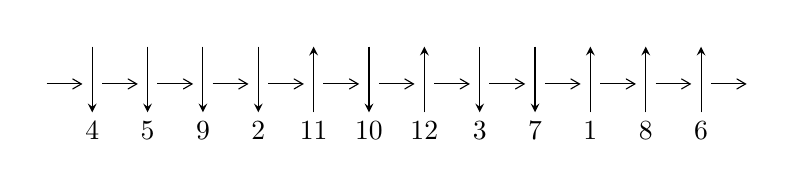
\begin{tikzpicture}[x=20pt, y=17pt]
	% nodes
	\node (C0) at (0, 0) {};
	\node (C1) at (1, 0) {};
	\node (C1U) at (1, +1) {};
	\node (C1D) at (1, -1) {4};

	\node (C2) at (2, 0) {};
	\node (C2U) at (2, +1) {};
	\node (C2D) at (2, -1) {5};

	\node (C3) at (3, 0) {};
	\node (C3U) at (3, +1) {};
	\node (C3D) at (3, -1) {9};

	\node (C4) at (4, 0) {};
	\node (C4U) at (4, +1) {};
	\node (C4D) at (4, -1) {2};

	\node (C5) at (5, 0) {};
	\node (C5U) at (5, +1) {};
	\node (C5D) at (5, -1) {11};

	\node (C6) at (6, 0) {};
	\node (C6U) at (6, +1) {};
	\node (C6D) at (6, -1) {10};

	\node (C7) at (7, 0) {};
	\node (C7U) at (7, +1) {};
	\node (C7D) at (7, -1) {12};

	\node (C8) at (8, 0) {};
	\node (C8U) at (8, +1) {};
	\node (C8D) at (8, -1) {3};

	\node (C9) at (9, 0) {};
	\node (C9U) at (9, +1) {};
	\node (C9D) at (9, -1) {7};

	\node (C10) at (10, 0) {};
	\node (C10U) at (10, +1) {};
	\node (C10D) at (10, -1) {1};

	\node (C11) at (11, 0) {};
	\node (C11U) at (11, +1) {};
	\node (C11D) at (11, -1) {8};

	\node (C12) at (12, 0) {};
	\node (C12U) at (12, +1) {};
	\node (C12D) at (12, -1) {6};
	\node (C13) at (13, 0) {};

	% arrows
	\draw[->,>={angle 60}]
	(C0) edge (C1) (C1) edge (C2) (C2) edge (C3) (C3) edge (C4) (C4) edge (C5) (C5) edge (C6) (C6) edge (C7) (C7) edge (C8) (C8) edge (C9) (C9) edge (C10) (C10) edge (C11) (C11) edge (C12) (C12) edge (C13) ;	\draw[->,>=stealth]
	(C1U) edge (C1D) (C2U) edge (C2D) (C3U) edge (C3D) (C4U) edge (C4D) (C5D) edge (C5U) (C6U) edge (C6D) (C7D) edge (C7U) (C8U) edge (C8D) (C9U) edge (C9D) (C10D) edge (C10U) (C11D) edge (C11U) (C12D) edge (C12U) ;
	\end{tikzpicture} \\
\hhline{~~} \\& 
\textbf{Solving Sequence} \\ \cline{2-2} 
 &
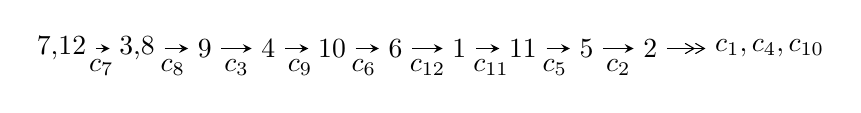
\begin{tikzpicture}[x=23pt, y=7pt]
	% node
	\node (A0) at (-1/8, 0) {7,12};
	\node (A1) at (17/16, 0) {3,8};
	\node (A2) at (17/8, 0) {9};
	\node (A3) at (25/8, 0) {4};
	\node (A4) at (33/8, 0) {10};
	\node (A5) at (41/8, 0) {6};
	\node (A6) at (49/8, 0) {1};
	\node (A7) at (57/8, 0) {11};
	\node (A8) at (65/8, 0) {5};
	\node (A9) at (73/8, 0) {2};
	\node (C1) at (1/2, -1) {$c_{7}$};
	\node (C2) at (13/8, -1) {$c_{8}$};
	\node (C3) at (21/8, -1) {$c_{3}$};
	\node (C4) at (29/8, -1) {$c_{9}$};
	\node (C5) at (37/8, -1) {$c_{6}$};
	\node (C6) at (45/8, -1) {$c_{12}$};
	\node (C7) at (53/8, -1) {$c_{11}$};
	\node (C8) at (61/8, -1) {$c_{5}$};
	\node (C9) at (69/8, -1) {$c_{2}$};
	\node (A10) at (11, 0) {$c_{1},c_{4},c_{10}$};

	% edge
	\draw[->,>=stealth]	
	(A0) edge (A1) (A1) edge (A2) (A2) edge (A3) (A3) edge (A4) (A4) edge (A5) (A5) edge (A6) (A6) edge (A7) (A7) edge (A8) (A8) edge (A9) ;
	\draw[->>,>={angle 60}]	
	(A9) edge (A10);
\end{tikzpicture} \\ 

\end{tabular} \\

\footnotetext{
The image of knot diagram is generated by the software ``\textbf{Draw programme}" developed by Andrew Bartholomew(\url{http://www.layer8.co.uk/maths/draw/index.htm\#Running-draw}), where we modified some parts for our purpose(\url{https://github.com/CATsTAILs/LinksPainter}).
}\phantom \\ \newline 
\centering \textbf{Ideals for irreducible components\footnotemark of $X_{\text{par}}$} 
 
\begin{align*}
I^u_{1}&=\langle 
7.31418\times10^{587} u^{129}+1.42814\times10^{588} u^{128}+\cdots+1.49614\times10^{590} b+2.54492\times10^{590},\\
\phantom{I^u_{1}}&\phantom{= \langle  }1.23726\times10^{589} u^{129}+1.96379\times10^{589} u^{128}+\cdots+3.44111\times10^{591} a+6.43358\times10^{592},\\
\phantom{I^u_{1}}&\phantom{= \langle  }u^{130}+2 u^{129}+\cdots+4232 u-4232\rangle \\
I^u_{2}&=\langle 
6 u^{19}+3 u^{18}+\cdots+b+13,\;-2 u^{19}+u^{18}+\cdots+a+2,\;u^{20}+10 u^{18}+\cdots+3 u+1\rangle \\
I^u_{3}&=\langle 
4 u^8+u^6+4 u^5+2 u^4+5 u^3- u^2+7 b- u+3,\\
\phantom{I^u_{3}}&\phantom{= \langle  }-4 u^8+7 u^7-15 u^6+10 u^5-16 u^4+9 u^3-13 u^2+7 a+u-3,\;u^9- u^8+2 u^7- u^6+3 u^5- u^4+2 u^3+u+1\rangle \\
\\
\end{align*}
\raggedright * 3 irreducible components of $\dim_{\mathbb{C}}=0$, with total 159 representations.\\
\footnotetext{All coefficients of polynomials are rational numbers. But the coefficients are sometimes approximated in decimal forms when there is not enough margin.}
\newpage
\renewcommand{\arraystretch}{1}
\centering \section*{I. $I^u_{1}= \langle 7.31\times10^{587} u^{129}+1.43\times10^{588} u^{128}+\cdots+1.50\times10^{590} b+2.54\times10^{590},\;1.24\times10^{589} u^{129}+1.96\times10^{589} u^{128}+\cdots+3.44\times10^{591} a+6.43\times10^{592},\;u^{130}+2 u^{129}+\cdots+4232 u-4232 \rangle$}
\flushleft \textbf{(i) Arc colorings}\\
\begin{tabular}{m{7pt} m{180pt} m{7pt} m{180pt} }
\flushright $a_{7}=$&$\begin{pmatrix}1\\0\end{pmatrix}$ \\
\flushright $a_{12}=$&$\begin{pmatrix}0\\u\end{pmatrix}$ \\
\flushright $a_{3}=$&$\begin{pmatrix}-0.00359551 u^{129}-0.00570685 u^{128}+\cdots+66.2600 u-18.6962\\-0.00488871 u^{129}-0.00954553 u^{128}+\cdots+62.4474 u-1.70099\end{pmatrix}$ \\
\flushright $a_{8}=$&$\begin{pmatrix}1\\- u^2\end{pmatrix}$ \\
\flushright $a_{9}=$&$\begin{pmatrix}0.000787540 u^{129}+0.00474240 u^{128}+\cdots+31.4660 u-17.0069\\0.00284266 u^{129}+0.00595084 u^{128}+\cdots+0.0159490 u-1.74523\end{pmatrix}$ \\
\flushright $a_{4}=$&$\begin{pmatrix}-0.00565176 u^{129}-0.00744750 u^{128}+\cdots+59.4935 u-12.5896\\-0.000553067 u^{129}-0.000371621 u^{128}+\cdots-1.21646 u+13.1924\end{pmatrix}$ \\
\flushright $a_{10}=$&$\begin{pmatrix}-0.00205512 u^{129}-0.00120844 u^{128}+\cdots+31.4501 u-15.2617\\0.00284266 u^{129}+0.00595084 u^{128}+\cdots+0.0159490 u-1.74523\end{pmatrix}$ \\
\flushright $a_{6}=$&$\begin{pmatrix}0.00535830 u^{129}+0.0124217 u^{128}+\cdots-21.2452 u-4.11354\\0.00265702 u^{129}+0.00676648 u^{128}+\cdots-32.0678 u+7.80220\end{pmatrix}$ \\
\flushright $a_{1}=$&$\begin{pmatrix}0.00169895 u^{129}+0.00692070 u^{128}+\cdots+8.87400 u-21.6666\\-0.00256817 u^{129}-0.00715091 u^{128}+\cdots+18.3812 u+9.46098\end{pmatrix}$ \\
\flushright $a_{11}=$&$\begin{pmatrix}- u\\u^3+u\end{pmatrix}$ \\
\flushright $a_{5}=$&$\begin{pmatrix}0.00831517 u^{129}+0.0204715 u^{128}+\cdots-31.2624 u-9.85356\\0.00238806 u^{129}+0.00614912 u^{128}+\cdots-25.5243 u+4.50253\end{pmatrix}$ \\
\flushright $a_{2}=$&$\begin{pmatrix}0.00237606 u^{129}+0.00902992 u^{128}+\cdots+13.9603 u-35.8227\\-0.00167924 u^{129}-0.00170185 u^{128}+\cdots+43.7419 u-26.9090\end{pmatrix}$\\&\end{tabular}
\flushleft \textbf{(ii) Obstruction class $= -1$}\\~\\
\flushleft \textbf{(iii) Cusp Shapes $= 0.0137665 u^{129}+0.0271520 u^{128}+\cdots-158.707 u-13.2029$}\\~\\
\newpage\renewcommand{\arraystretch}{1}
\flushleft \textbf{(iv) u-Polynomials at the component}\newline \\
\begin{tabular}{m{50pt}|m{274pt}}
Crossings & \hspace{64pt}u-Polynomials at each crossing \\
\hline $$\begin{aligned}c_{1},c_{2},c_{4}\end{aligned}$$&$\begin{aligned}
&u^{130}-14 u^{129}+\cdots+35 u-49
\end{aligned}$\\
\hline $$\begin{aligned}c_{3},c_{8}\end{aligned}$$&$\begin{aligned}
&u^{130}+u^{129}+\cdots-60928 u+25088
\end{aligned}$\\
\hline $$\begin{aligned}c_{5}\end{aligned}$$&$\begin{aligned}
&u^{130}+u^{129}+\cdots-15153510 u-893777
\end{aligned}$\\
\hline $$\begin{aligned}c_{6},c_{9}\end{aligned}$$&$\begin{aligned}
&u^{130}-3 u^{129}+\cdots+4534 u-71
\end{aligned}$\\
\hline $$\begin{aligned}c_{7},c_{11}\end{aligned}$$&$\begin{aligned}
&u^{130}-2 u^{129}+\cdots-4232 u-4232
\end{aligned}$\\
\hline $$\begin{aligned}c_{10}\end{aligned}$$&$\begin{aligned}
&u^{130}+18 u^{129}+\cdots-8409 u+1079
\end{aligned}$\\
\hline $$\begin{aligned}c_{12}\end{aligned}$$&$\begin{aligned}
&u^{130}+10 u^{129}+\cdots-27 u-9
\end{aligned}$\\
\hline
\end{tabular}\\~\\
\newpage\renewcommand{\arraystretch}{1}
\flushleft \textbf{(v) Riley Polynomials at the component}\newline \\
\begin{tabular}{m{50pt}|m{274pt}}
Crossings & \hspace{64pt}Riley Polynomials at each crossing \\
\hline $$\begin{aligned}c_{1},c_{2},c_{4}\end{aligned}$$&$\begin{aligned}
&y^{130}-122 y^{129}+\cdots-5929 y+2401
\end{aligned}$\\
\hline $$\begin{aligned}c_{3},c_{8}\end{aligned}$$&$\begin{aligned}
&y^{130}-69 y^{129}+\cdots-11984437248 y+629407744
\end{aligned}$\\
\hline $$\begin{aligned}c_{5}\end{aligned}$$&$\begin{aligned}
&y^{130}+13 y^{129}+\cdots+20581982318772 y+798837325729
\end{aligned}$\\
\hline $$\begin{aligned}c_{6},c_{9}\end{aligned}$$&$\begin{aligned}
&y^{130}+81 y^{129}+\cdots-16239788 y+5041
\end{aligned}$\\
\hline $$\begin{aligned}c_{7},c_{11}\end{aligned}$$&$\begin{aligned}
&y^{130}+86 y^{129}+\cdots+519774240 y+17909824
\end{aligned}$\\
\hline $$\begin{aligned}c_{10}\end{aligned}$$&$\begin{aligned}
&y^{130}-26 y^{129}+\cdots-102045441 y+1164241
\end{aligned}$\\
\hline $$\begin{aligned}c_{12}\end{aligned}$$&$\begin{aligned}
&y^{130}-6 y^{129}+\cdots+2151 y+81
\end{aligned}$\\
\hline
\end{tabular}\\~\\
\newpage\flushleft \textbf{(vi) Complex Volumes and Cusp Shapes}
$$\begin{array}{c|c|c}  
\text{Solutions to }I^u_{1}& \I (\text{vol} + \sqrt{-1}CS) & \text{Cusp shape}\\
 \hline 
\begin{aligned}
u &= -0.207403 + 0.977252 I \\
a &= -2.13432 + 1.44213 I \\
b &= -1.29939 + 0.83567 I\end{aligned}
 & -5.39383 - 0.67456 I & \phantom{-0.000000 } 0 \\ \hline\begin{aligned}
u &= -0.207403 - 0.977252 I \\
a &= -2.13432 - 1.44213 I \\
b &= -1.29939 - 0.83567 I\end{aligned}
 & -5.39383 + 0.67456 I & \phantom{-0.000000 } 0 \\ \hline\begin{aligned}
u &= \phantom{-}0.870481 + 0.482230 I \\
a &= \phantom{-}0.136852 + 0.115419 I \\
b &= -1.231720 - 0.550774 I\end{aligned}
 & -7.57713 - 2.60992 I & \phantom{-0.000000 } 0 \\ \hline\begin{aligned}
u &= \phantom{-}0.870481 - 0.482230 I \\
a &= \phantom{-}0.136852 - 0.115419 I \\
b &= -1.231720 + 0.550774 I\end{aligned}
 & -7.57713 + 2.60992 I & \phantom{-0.000000 } 0 \\ \hline\begin{aligned}
u &= -0.207306 + 0.968285 I \\
a &= \phantom{-}0.552789 - 1.258600 I \\
b &= \phantom{-}0.851569 - 0.056422 I\end{aligned}
 & -1.20363 - 3.45389 I & \phantom{-0.000000 } 0 \\ \hline\begin{aligned}
u &= -0.207306 - 0.968285 I \\
a &= \phantom{-}0.552789 + 1.258600 I \\
b &= \phantom{-}0.851569 + 0.056422 I\end{aligned}
 & -1.20363 + 3.45389 I & \phantom{-0.000000 } 0 \\ \hline\begin{aligned}
u &= \phantom{-}0.045460 + 0.986316 I \\
a &= \phantom{-}0.031164 + 1.041930 I \\
b &= \phantom{-}0.420336 - 0.550031 I\end{aligned}
 & -4.06225 + 0.19731 I & \phantom{-0.000000 } 0 \\ \hline\begin{aligned}
u &= \phantom{-}0.045460 - 0.986316 I \\
a &= \phantom{-}0.031164 - 1.041930 I \\
b &= \phantom{-}0.420336 + 0.550031 I\end{aligned}
 & -4.06225 - 0.19731 I & \phantom{-0.000000 } 0 \\ \hline\begin{aligned}
u &= \phantom{-}0.355513 + 0.900991 I \\
a &= \phantom{-}0.542870 - 0.433386 I \\
b &= -0.353756 + 0.490944 I\end{aligned}
 & \phantom{-}3.12587 + 4.37430 I & \phantom{-0.000000 } 0 \\ \hline\begin{aligned}
u &= \phantom{-}0.355513 - 0.900991 I \\
a &= \phantom{-}0.542870 + 0.433386 I \\
b &= -0.353756 - 0.490944 I\end{aligned}
 & \phantom{-}3.12587 - 4.37430 I & \phantom{-0.000000 } 0\\
 \hline 
 \end{array}$$\newpage$$\begin{array}{c|c|c}  
\text{Solutions to }I^u_{1}& \I (\text{vol} + \sqrt{-1}CS) & \text{Cusp shape}\\
 \hline 
\begin{aligned}
u &= \phantom{-}0.052715 + 1.033720 I \\
a &= -0.288223 + 0.352604 I \\
b &= \phantom{-}0.134358 + 0.922567 I\end{aligned}
 & -1.62444 - 1.37557 I & \phantom{-0.000000 } 0 \\ \hline\begin{aligned}
u &= \phantom{-}0.052715 - 1.033720 I \\
a &= -0.288223 - 0.352604 I \\
b &= \phantom{-}0.134358 - 0.922567 I\end{aligned}
 & -1.62444 + 1.37557 I & \phantom{-0.000000 } 0 \\ \hline\begin{aligned}
u &= -0.959148 + 0.078977 I \\
a &= \phantom{-}1.057860 - 0.294072 I \\
b &= -1.78753 + 0.77001 I\end{aligned}
 & \phantom{-}1.39635 + 3.23709 I & \phantom{-0.000000 } 0 \\ \hline\begin{aligned}
u &= -0.959148 - 0.078977 I \\
a &= \phantom{-}1.057860 + 0.294072 I \\
b &= -1.78753 - 0.77001 I\end{aligned}
 & \phantom{-}1.39635 - 3.23709 I & \phantom{-0.000000 } 0 \\ \hline\begin{aligned}
u &= -0.140669 + 1.028800 I \\
a &= -2.12933 - 0.04020 I \\
b &= -0.645111 - 0.983937 I\end{aligned}
 & -2.45297 - 3.70553 I & \phantom{-0.000000 } 0 \\ \hline\begin{aligned}
u &= -0.140669 - 1.028800 I \\
a &= -2.12933 + 0.04020 I \\
b &= -0.645111 + 0.983937 I\end{aligned}
 & -2.45297 + 3.70553 I & \phantom{-0.000000 } 0 \\ \hline\begin{aligned}
u &= \phantom{-}0.523222 + 0.802656 I \\
a &= \phantom{-}2.49879 + 4.67344 I \\
b &= \phantom{-}4.65998 + 0.06588 I\end{aligned}
 & -0.42547 + 2.53758 I & \phantom{-0.000000 } 0 \\ \hline\begin{aligned}
u &= \phantom{-}0.523222 - 0.802656 I \\
a &= \phantom{-}2.49879 - 4.67344 I \\
b &= \phantom{-}4.65998 - 0.06588 I\end{aligned}
 & -0.42547 - 2.53758 I & \phantom{-0.000000 } 0 \\ \hline\begin{aligned}
u &= \phantom{-}0.309325 + 0.872790 I \\
a &= -2.03045 - 1.07152 I \\
b &= -0.499650 - 0.281157 I\end{aligned}
 & -8.13468 + 7.32693 I & \phantom{-0.000000 } 0 \\ \hline\begin{aligned}
u &= \phantom{-}0.309325 - 0.872790 I \\
a &= -2.03045 + 1.07152 I \\
b &= -0.499650 + 0.281157 I\end{aligned}
 & -8.13468 - 7.32693 I & \phantom{-0.000000 } 0\\
 \hline 
 \end{array}$$\newpage$$\begin{array}{c|c|c}  
\text{Solutions to }I^u_{1}& \I (\text{vol} + \sqrt{-1}CS) & \text{Cusp shape}\\
 \hline 
\begin{aligned}
u &= \phantom{-}1.009940 + 0.380275 I \\
a &= -0.749459 - 0.478953 I \\
b &= \phantom{-}0.790741 + 0.283640 I\end{aligned}
 & \phantom{-}5.03065 - 2.91197 I & \phantom{-0.000000 } 0 \\ \hline\begin{aligned}
u &= \phantom{-}1.009940 - 0.380275 I \\
a &= -0.749459 + 0.478953 I \\
b &= \phantom{-}0.790741 - 0.283640 I\end{aligned}
 & \phantom{-}5.03065 + 2.91197 I & \phantom{-0.000000 } 0 \\ \hline\begin{aligned}
u &= \phantom{-}0.556506 + 0.727484 I \\
a &= \phantom{-}0.297857 - 0.675164 I \\
b &= -0.389439 + 0.331391 I\end{aligned}
 & \phantom{-}3.62319 - 0.56871 I & \phantom{-0.000000 } 0 \\ \hline\begin{aligned}
u &= \phantom{-}0.556506 - 0.727484 I \\
a &= \phantom{-}0.297857 + 0.675164 I \\
b &= -0.389439 - 0.331391 I\end{aligned}
 & \phantom{-}3.62319 + 0.56871 I & \phantom{-0.000000 } 0 \\ \hline\begin{aligned}
u &= -0.541139 + 0.952132 I \\
a &= \phantom{-}0.147250 + 0.918610 I \\
b &= -0.178510 + 0.299329 I\end{aligned}
 & \phantom{-}1.88655 - 1.65023 I & \phantom{-0.000000 } 0 \\ \hline\begin{aligned}
u &= -0.541139 - 0.952132 I \\
a &= \phantom{-}0.147250 - 0.918610 I \\
b &= -0.178510 - 0.299329 I\end{aligned}
 & \phantom{-}1.88655 + 1.65023 I & \phantom{-0.000000 } 0 \\ \hline\begin{aligned}
u &= -0.290943 + 1.071750 I \\
a &= \phantom{-}0.359265 + 0.121506 I \\
b &= \phantom{-}0.669032 - 0.344390 I\end{aligned}
 & -1.67452 - 3.13091 I & \phantom{-0.000000 } 0 \\ \hline\begin{aligned}
u &= -0.290943 - 1.071750 I \\
a &= \phantom{-}0.359265 - 0.121506 I \\
b &= \phantom{-}0.669032 + 0.344390 I\end{aligned}
 & -1.67452 + 3.13091 I & \phantom{-0.000000 } 0 \\ \hline\begin{aligned}
u &= \phantom{-}0.296795 + 1.075410 I \\
a &= -2.91041 - 0.47249 I \\
b &= -2.50052 + 0.95290 I\end{aligned}
 & \phantom{-}1.16491 + 5.17903 I & \phantom{-0.000000 } 0 \\ \hline\begin{aligned}
u &= \phantom{-}0.296795 - 1.075410 I \\
a &= -2.91041 + 0.47249 I \\
b &= -2.50052 - 0.95290 I\end{aligned}
 & \phantom{-}1.16491 - 5.17903 I & \phantom{-0.000000 } 0\\
 \hline 
 \end{array}$$\newpage$$\begin{array}{c|c|c}  
\text{Solutions to }I^u_{1}& \I (\text{vol} + \sqrt{-1}CS) & \text{Cusp shape}\\
 \hline 
\begin{aligned}
u &= -0.750310 + 0.427363 I \\
a &= \phantom{-}0.068052 + 0.564511 I \\
b &= \phantom{-}0.697843 + 0.441677 I\end{aligned}
 & -1.53269 - 6.33362 I & \phantom{-0.000000 } 0 \\ \hline\begin{aligned}
u &= -0.750310 - 0.427363 I \\
a &= \phantom{-}0.068052 - 0.564511 I \\
b &= \phantom{-}0.697843 - 0.441677 I\end{aligned}
 & -1.53269 + 6.33362 I & \phantom{-0.000000 } 0 \\ \hline\begin{aligned}
u &= \phantom{-}0.016383 + 0.861091 I \\
a &= \phantom{-}2.51607 + 0.55432 I \\
b &= \phantom{-}0.481827 + 0.674512 I\end{aligned}
 & -1.42660 + 2.83814 I & \phantom{-0.000000 } 0 \\ \hline\begin{aligned}
u &= \phantom{-}0.016383 - 0.861091 I \\
a &= \phantom{-}2.51607 - 0.55432 I \\
b &= \phantom{-}0.481827 - 0.674512 I\end{aligned}
 & -1.42660 - 2.83814 I & \phantom{-0.000000 } 0 \\ \hline\begin{aligned}
u &= -0.666858 + 0.939090 I \\
a &= -0.214878 + 0.171005 I \\
b &= -0.409765 + 0.257143 I\end{aligned}
 & \phantom{-}0.38694 - 2.59415 I & \phantom{-0.000000 } 0 \\ \hline\begin{aligned}
u &= -0.666858 - 0.939090 I \\
a &= -0.214878 - 0.171005 I \\
b &= -0.409765 - 0.257143 I\end{aligned}
 & \phantom{-}0.38694 + 2.59415 I & \phantom{-0.000000 } 0 \\ \hline\begin{aligned}
u &= \phantom{-}1.172230 + 0.057028 I \\
a &= \phantom{-}0.688708 + 1.000700 I \\
b &= -1.222240 - 0.451724 I\end{aligned}
 & \phantom{-}0.47369 - 5.68832 I & \phantom{-0.000000 } 0 \\ \hline\begin{aligned}
u &= \phantom{-}1.172230 - 0.057028 I \\
a &= \phantom{-}0.688708 - 1.000700 I \\
b &= -1.222240 + 0.451724 I\end{aligned}
 & \phantom{-}0.47369 + 5.68832 I & \phantom{-0.000000 } 0 \\ \hline\begin{aligned}
u &= -0.646682 + 0.508924 I \\
a &= -0.607220 + 0.928340 I \\
b &= -1.117150 - 0.578316 I\end{aligned}
 & \phantom{-}0.75859 - 3.24972 I & \phantom{-0.000000 } 0 \\ \hline\begin{aligned}
u &= -0.646682 - 0.508924 I \\
a &= -0.607220 - 0.928340 I \\
b &= -1.117150 + 0.578316 I\end{aligned}
 & \phantom{-}0.75859 + 3.24972 I & \phantom{-0.000000 } 0\\
 \hline 
 \end{array}$$\newpage$$\begin{array}{c|c|c}  
\text{Solutions to }I^u_{1}& \I (\text{vol} + \sqrt{-1}CS) & \text{Cusp shape}\\
 \hline 
\begin{aligned}
u &= -0.306526 + 0.755382 I \\
a &= -0.326678 - 0.381872 I \\
b &= -0.881679 - 0.168136 I\end{aligned}
 & -4.78653 - 1.59407 I & \phantom{-0.000000 } 0 \\ \hline\begin{aligned}
u &= -0.306526 - 0.755382 I \\
a &= -0.326678 + 0.381872 I \\
b &= -0.881679 + 0.168136 I\end{aligned}
 & -4.78653 + 1.59407 I & \phantom{-0.000000 } 0 \\ \hline\begin{aligned}
u &= \phantom{-}0.788563 + 0.204340 I \\
a &= \phantom{-}0.534729 + 0.656471 I \\
b &= \phantom{-}1.170900 - 0.040856 I\end{aligned}
 & -6.57708 - 7.15153 I & \phantom{-0.000000 } 0 \\ \hline\begin{aligned}
u &= \phantom{-}0.788563 - 0.204340 I \\
a &= \phantom{-}0.534729 - 0.656471 I \\
b &= \phantom{-}1.170900 + 0.040856 I\end{aligned}
 & -6.57708 + 7.15153 I & \phantom{-0.000000 } 0 \\ \hline\begin{aligned}
u &= \phantom{-}0.067187 + 0.805703 I \\
a &= \phantom{-}3.65880 - 1.74203 I \\
b &= \phantom{-}1.37055 - 1.72420 I\end{aligned}
 & \phantom{-}0.47179 + 1.76850 I & \phantom{-0.000000 } 0 \\ \hline\begin{aligned}
u &= \phantom{-}0.067187 - 0.805703 I \\
a &= \phantom{-}3.65880 + 1.74203 I \\
b &= \phantom{-}1.37055 + 1.72420 I\end{aligned}
 & \phantom{-}0.47179 - 1.76850 I & \phantom{-0.000000 } 0 \\ \hline\begin{aligned}
u &= \phantom{-}0.071155 + 1.217340 I \\
a &= \phantom{-}1.093210 + 0.732066 I \\
b &= \phantom{-}0.782484 - 0.448149 I\end{aligned}
 & -4.64544 + 1.87466 I & \phantom{-0.000000 } 0 \\ \hline\begin{aligned}
u &= \phantom{-}0.071155 - 1.217340 I \\
a &= \phantom{-}1.093210 - 0.732066 I \\
b &= \phantom{-}0.782484 + 0.448149 I\end{aligned}
 & -4.64544 - 1.87466 I & \phantom{-0.000000 } 0 \\ \hline\begin{aligned}
u &= -0.220315 + 1.200090 I \\
a &= -1.96529 - 0.03345 I \\
b &= -1.327500 - 0.345449 I\end{aligned}
 & -0.99196 - 4.71706 I & \phantom{-0.000000 } 0 \\ \hline\begin{aligned}
u &= -0.220315 - 1.200090 I \\
a &= -1.96529 + 0.03345 I \\
b &= -1.327500 + 0.345449 I\end{aligned}
 & -0.99196 + 4.71706 I & \phantom{-0.000000 } 0\\
 \hline 
 \end{array}$$\newpage$$\begin{array}{c|c|c}  
\text{Solutions to }I^u_{1}& \I (\text{vol} + \sqrt{-1}CS) & \text{Cusp shape}\\
 \hline 
\begin{aligned}
u &= \phantom{-}0.813144 + 0.914977 I \\
a &= -0.183806 - 0.173935 I \\
b &= \phantom{-}0.358860 + 0.079720 I\end{aligned}
 & \phantom{-}1.52846 + 7.35278 I & \phantom{-0.000000 } 0 \\ \hline\begin{aligned}
u &= \phantom{-}0.813144 - 0.914977 I \\
a &= -0.183806 + 0.173935 I \\
b &= \phantom{-}0.358860 - 0.079720 I\end{aligned}
 & \phantom{-}1.52846 - 7.35278 I & \phantom{-0.000000 } 0 \\ \hline\begin{aligned}
u &= -0.759942\phantom{ +0.000000I} \\
a &= \phantom{-}0.944622\phantom{ +0.000000I} \\
b &= \phantom{-}0.523634\phantom{ +0.000000I}\end{aligned}
 & -2.56238\phantom{ +0.000000I} & -1.14050\phantom{ +0.000000I} \\ \hline\begin{aligned}
u &= \phantom{-}0.010388 + 1.247310 I \\
a &= \phantom{-}1.65859 - 0.36936 I \\
b &= \phantom{-}1.80529 - 1.08613 I\end{aligned}
 & -4.78176 + 1.13220 I & \phantom{-0.000000 } 0 \\ \hline\begin{aligned}
u &= \phantom{-}0.010388 - 1.247310 I \\
a &= \phantom{-}1.65859 + 0.36936 I \\
b &= \phantom{-}1.80529 + 1.08613 I\end{aligned}
 & -4.78176 - 1.13220 I & \phantom{-0.000000 } 0 \\ \hline\begin{aligned}
u &= -0.721881 + 1.025220 I \\
a &= -0.015244 - 0.728804 I \\
b &= -0.0448569 - 0.0263149 I\end{aligned}
 & -3.08113 + 0.81431 I & \phantom{-0.000000 } 0 \\ \hline\begin{aligned}
u &= -0.721881 - 1.025220 I \\
a &= -0.015244 + 0.728804 I \\
b &= -0.0448569 + 0.0263149 I\end{aligned}
 & -3.08113 - 0.81431 I & \phantom{-0.000000 } 0 \\ \hline\begin{aligned}
u &= \phantom{-}0.309343 + 1.237480 I \\
a &= \phantom{-}1.89400 + 0.83926 I \\
b &= \phantom{-}2.28057 - 0.00970 I\end{aligned}
 & -5.66140 + 2.87702 I & \phantom{-0.000000 } 0 \\ \hline\begin{aligned}
u &= \phantom{-}0.309343 - 1.237480 I \\
a &= \phantom{-}1.89400 - 0.83926 I \\
b &= \phantom{-}2.28057 + 0.00970 I\end{aligned}
 & -5.66140 - 2.87702 I & \phantom{-0.000000 } 0 \\ \hline\begin{aligned}
u &= \phantom{-}0.265868 + 1.248280 I \\
a &= \phantom{-}2.24133 + 0.22130 I \\
b &= \phantom{-}2.26417 - 0.63628 I\end{aligned}
 & -4.41116 + 8.47604 I & \phantom{-0.000000 } 0\\
 \hline 
 \end{array}$$\newpage$$\begin{array}{c|c|c}  
\text{Solutions to }I^u_{1}& \I (\text{vol} + \sqrt{-1}CS) & \text{Cusp shape}\\
 \hline 
\begin{aligned}
u &= \phantom{-}0.265868 - 1.248280 I \\
a &= \phantom{-}2.24133 - 0.22130 I \\
b &= \phantom{-}2.26417 + 0.63628 I\end{aligned}
 & -4.41116 - 8.47604 I & \phantom{-0.000000 } 0 \\ \hline\begin{aligned}
u &= -1.274750 + 0.149399 I \\
a &= -0.629685 - 0.215734 I \\
b &= \phantom{-}2.13894 - 0.43531 I\end{aligned}
 & \phantom{-}3.35673 + 7.72625 I & \phantom{-0.000000 } 0 \\ \hline\begin{aligned}
u &= -1.274750 - 0.149399 I \\
a &= -0.629685 + 0.215734 I \\
b &= \phantom{-}2.13894 + 0.43531 I\end{aligned}
 & \phantom{-}3.35673 - 7.72625 I & \phantom{-0.000000 } 0 \\ \hline\begin{aligned}
u &= \phantom{-}0.439475 + 1.206410 I \\
a &= -1.61258 - 1.11031 I \\
b &= -2.07853 - 0.22200 I\end{aligned}
 & -4.00841 + 7.89339 I & \phantom{-0.000000 } 0 \\ \hline\begin{aligned}
u &= \phantom{-}0.439475 - 1.206410 I \\
a &= -1.61258 + 1.11031 I \\
b &= -2.07853 + 0.22200 I\end{aligned}
 & -4.00841 - 7.89339 I & \phantom{-0.000000 } 0 \\ \hline\begin{aligned}
u &= \phantom{-}0.596326 + 1.151090 I \\
a &= -0.118605 + 0.317783 I \\
b &= \phantom{-}0.077208 - 0.472785 I\end{aligned}
 & \phantom{-}2.56590 + 8.61563 I & \phantom{-0.000000 } 0 \\ \hline\begin{aligned}
u &= \phantom{-}0.596326 - 1.151090 I \\
a &= -0.118605 - 0.317783 I \\
b &= \phantom{-}0.077208 + 0.472785 I\end{aligned}
 & \phantom{-}2.56590 - 8.61563 I & \phantom{-0.000000 } 0 \\ \hline\begin{aligned}
u &= -0.385070 + 1.240120 I \\
a &= -0.444387 - 0.153876 I \\
b &= -0.861742 + 0.514358 I\end{aligned}
 & -6.87980 - 5.59995 I & \phantom{-0.000000 } 0 \\ \hline\begin{aligned}
u &= -0.385070 - 1.240120 I \\
a &= -0.444387 + 0.153876 I \\
b &= -0.861742 - 0.514358 I\end{aligned}
 & -6.87980 + 5.59995 I & \phantom{-0.000000 } 0 \\ \hline\begin{aligned}
u &= \phantom{-}1.050980 + 0.804516 I \\
a &= \phantom{-}0.321098 + 0.405591 I \\
b &= -0.288639 - 0.548025 I\end{aligned}
 & \phantom{-}1.95452 - 0.73217 I & \phantom{-0.000000 } 0\\
 \hline 
 \end{array}$$\newpage$$\begin{array}{c|c|c}  
\text{Solutions to }I^u_{1}& \I (\text{vol} + \sqrt{-1}CS) & \text{Cusp shape}\\
 \hline 
\begin{aligned}
u &= \phantom{-}1.050980 - 0.804516 I \\
a &= \phantom{-}0.321098 - 0.405591 I \\
b &= -0.288639 + 0.548025 I\end{aligned}
 & \phantom{-}1.95452 + 0.73217 I & \phantom{-0.000000 } 0 \\ \hline\begin{aligned}
u &= \phantom{-}0.297996 + 0.596894 I \\
a &= -0.54817 + 1.51250 I \\
b &= \phantom{-}1.05023 + 1.30928 I\end{aligned}
 & -0.131132 + 1.178100 I & -1.130855 - 0.687358 I \\ \hline\begin{aligned}
u &= \phantom{-}0.297996 - 0.596894 I \\
a &= -0.54817 - 1.51250 I \\
b &= \phantom{-}1.05023 - 1.30928 I\end{aligned}
 & -0.131132 - 1.178100 I & -1.130855 + 0.687358 I \\ \hline\begin{aligned}
u &= \phantom{-}0.537857 + 1.232880 I \\
a &= \phantom{-}1.39056 + 1.09863 I \\
b &= \phantom{-}1.89489 + 0.20264 I\end{aligned}
 & -9.7181 + 12.1998 I & \phantom{-0.000000 } 0 \\ \hline\begin{aligned}
u &= \phantom{-}0.537857 - 1.232880 I \\
a &= \phantom{-}1.39056 - 1.09863 I \\
b &= \phantom{-}1.89489 - 0.20264 I\end{aligned}
 & -9.7181 - 12.1998 I & \phantom{-0.000000 } 0 \\ \hline\begin{aligned}
u &= -0.447868 + 0.446054 I \\
a &= -0.179300 - 0.673744 I \\
b &= -0.583300 - 0.734247 I\end{aligned}
 & \phantom{-}3.14662 - 2.57828 I & \phantom{-}3.70857 + 3.51309 I \\ \hline\begin{aligned}
u &= -0.447868 - 0.446054 I \\
a &= -0.179300 + 0.673744 I \\
b &= -0.583300 + 0.734247 I\end{aligned}
 & \phantom{-}3.14662 + 2.57828 I & \phantom{-}3.70857 - 3.51309 I \\ \hline\begin{aligned}
u &= -0.619320 + 0.098741 I \\
a &= \phantom{-}0.64193 - 1.63021 I \\
b &= \phantom{-}0.111781 - 0.294175 I\end{aligned}
 & -2.97910 - 1.77302 I & -5.16591 + 3.41651 I \\ \hline\begin{aligned}
u &= -0.619320 - 0.098741 I \\
a &= \phantom{-}0.64193 + 1.63021 I \\
b &= \phantom{-}0.111781 + 0.294175 I\end{aligned}
 & -2.97910 + 1.77302 I & -5.16591 - 3.41651 I \\ \hline\begin{aligned}
u &= -0.246238 + 1.353050 I \\
a &= \phantom{-}1.73313 - 0.06279 I \\
b &= \phantom{-}1.43771 + 0.98489 I\end{aligned}
 & -12.25150 - 6.55987 I & \phantom{-0.000000 } 0\\
 \hline 
 \end{array}$$\newpage$$\begin{array}{c|c|c}  
\text{Solutions to }I^u_{1}& \I (\text{vol} + \sqrt{-1}CS) & \text{Cusp shape}\\
 \hline 
\begin{aligned}
u &= -0.246238 - 1.353050 I \\
a &= \phantom{-}1.73313 + 0.06279 I \\
b &= \phantom{-}1.43771 - 0.98489 I\end{aligned}
 & -12.25150 + 6.55987 I & \phantom{-0.000000 } 0 \\ \hline\begin{aligned}
u &= -0.329709 + 1.346510 I \\
a &= \phantom{-}1.69685 - 0.19298 I \\
b &= \phantom{-}1.74640 + 0.33574 I\end{aligned}
 & -6.71754 - 9.96409 I & \phantom{-0.000000 } 0 \\ \hline\begin{aligned}
u &= -0.329709 - 1.346510 I \\
a &= \phantom{-}1.69685 + 0.19298 I \\
b &= \phantom{-}1.74640 - 0.33574 I\end{aligned}
 & -6.71754 + 9.96409 I & \phantom{-0.000000 } 0 \\ \hline\begin{aligned}
u &= \phantom{-}0.615817 + 1.246730 I \\
a &= -1.61173 - 0.21772 I \\
b &= -1.13458 + 2.31191 I\end{aligned}
 & -2.89630 + 0.85409 I & \phantom{-0.000000 } 0 \\ \hline\begin{aligned}
u &= \phantom{-}0.615817 - 1.246730 I \\
a &= -1.61173 + 0.21772 I \\
b &= -1.13458 - 2.31191 I\end{aligned}
 & -2.89630 - 0.85409 I & \phantom{-0.000000 } 0 \\ \hline\begin{aligned}
u &= \phantom{-}0.599539 + 0.031257 I \\
a &= -0.134478 - 1.293650 I \\
b &= -1.000210 + 0.123339 I\end{aligned}
 & -0.63869 - 3.79000 I & -3.28691 + 6.67650 I \\ \hline\begin{aligned}
u &= \phantom{-}0.599539 - 0.031257 I \\
a &= -0.134478 + 1.293650 I \\
b &= -1.000210 - 0.123339 I\end{aligned}
 & -0.63869 + 3.79000 I & -3.28691 - 6.67650 I \\ \hline\begin{aligned}
u &= -0.526568 + 1.297290 I \\
a &= -1.84964 + 0.47697 I \\
b &= -1.97035 - 1.49638 I\end{aligned}
 & -2.38605 - 8.61930 I & \phantom{-0.000000 } 0 \\ \hline\begin{aligned}
u &= -0.526568 - 1.297290 I \\
a &= -1.84964 - 0.47697 I \\
b &= -1.97035 + 1.49638 I\end{aligned}
 & -2.38605 + 8.61930 I & \phantom{-0.000000 } 0 \\ \hline\begin{aligned}
u &= -1.281120 + 0.570799 I \\
a &= -0.023425 - 0.158691 I \\
b &= \phantom{-}1.51149 - 0.04289 I\end{aligned}
 & -5.37237 - 2.41269 I & \phantom{-0.000000 } 0\\
 \hline 
 \end{array}$$\newpage$$\begin{array}{c|c|c}  
\text{Solutions to }I^u_{1}& \I (\text{vol} + \sqrt{-1}CS) & \text{Cusp shape}\\
 \hline 
\begin{aligned}
u &= -1.281120 - 0.570799 I \\
a &= -0.023425 + 0.158691 I \\
b &= \phantom{-}1.51149 + 0.04289 I\end{aligned}
 & -5.37237 + 2.41269 I & \phantom{-0.000000 } 0 \\ \hline\begin{aligned}
u &= \phantom{-}0.527514 + 0.253658 I \\
a &= -0.797736 - 0.405039 I \\
b &= \phantom{-}0.920390 + 0.384396 I\end{aligned}
 & -1.385150 - 0.269456 I & -6.74039 + 0.20784 I \\ \hline\begin{aligned}
u &= \phantom{-}0.527514 - 0.253658 I \\
a &= -0.797736 + 0.405039 I \\
b &= \phantom{-}0.920390 - 0.384396 I\end{aligned}
 & -1.385150 + 0.269456 I & -6.74039 - 0.20784 I \\ \hline\begin{aligned}
u &= -0.40824 + 1.38572 I \\
a &= -1.26301 + 0.82009 I \\
b &= -2.21976 + 0.37082 I\end{aligned}
 & -2.96488 - 2.11966 I & \phantom{-0.000000 } 0 \\ \hline\begin{aligned}
u &= -0.40824 - 1.38572 I \\
a &= -1.26301 - 0.82009 I \\
b &= -2.21976 - 0.37082 I\end{aligned}
 & -2.96488 + 2.11966 I & \phantom{-0.000000 } 0 \\ \hline\begin{aligned}
u &= -0.73422 + 1.25225 I \\
a &= \phantom{-}0.343833 - 0.161391 I \\
b &= \phantom{-}0.770766 - 0.683082 I\end{aligned}
 & -4.71583 - 3.31857 I & \phantom{-0.000000 } 0 \\ \hline\begin{aligned}
u &= -0.73422 - 1.25225 I \\
a &= \phantom{-}0.343833 + 0.161391 I \\
b &= \phantom{-}0.770766 + 0.683082 I\end{aligned}
 & -4.71583 + 3.31857 I & \phantom{-0.000000 } 0 \\ \hline\begin{aligned}
u &= -0.152962 + 0.522678 I \\
a &= \phantom{-}0.052409 + 1.203110 I \\
b &= \phantom{-}0.483156 + 1.065560 I\end{aligned}
 & -0.169062 + 1.292200 I & -1.82953 + 1.55175 I \\ \hline\begin{aligned}
u &= -0.152962 - 0.522678 I \\
a &= \phantom{-}0.052409 - 1.203110 I \\
b &= \phantom{-}0.483156 - 1.065560 I\end{aligned}
 & -0.169062 - 1.292200 I & -1.82953 - 1.55175 I \\ \hline\begin{aligned}
u &= \phantom{-}0.57273 + 1.34557 I \\
a &= \phantom{-}0.043546 - 0.393122 I \\
b &= -0.046931 + 0.648616 I\end{aligned}
 & -3.56917 + 11.75340 I & \phantom{-0.000000 } 0\\
 \hline 
 \end{array}$$\newpage$$\begin{array}{c|c|c}  
\text{Solutions to }I^u_{1}& \I (\text{vol} + \sqrt{-1}CS) & \text{Cusp shape}\\
 \hline 
\begin{aligned}
u &= \phantom{-}0.57273 - 1.34557 I \\
a &= \phantom{-}0.043546 + 0.393122 I \\
b &= -0.046931 - 0.648616 I\end{aligned}
 & -3.56917 - 11.75340 I & \phantom{-0.000000 } 0 \\ \hline\begin{aligned}
u &= \phantom{-}0.21861 + 1.45249 I \\
a &= -1.55078 - 0.43115 I \\
b &= -1.99666 + 0.19901 I\end{aligned}
 & -13.95940 + 1.16927 I & \phantom{-0.000000 } 0 \\ \hline\begin{aligned}
u &= \phantom{-}0.21861 - 1.45249 I \\
a &= -1.55078 + 0.43115 I \\
b &= -1.99666 - 0.19901 I\end{aligned}
 & -13.95940 - 1.16927 I & \phantom{-0.000000 } 0 \\ \hline\begin{aligned}
u &= -1.46184 + 0.14608 I \\
a &= \phantom{-}0.403978 + 0.285131 I \\
b &= -2.20414 + 0.22320 I\end{aligned}
 & -2.13477 + 11.78310 I & \phantom{-0.000000 } 0 \\ \hline\begin{aligned}
u &= -1.46184 - 0.14608 I \\
a &= \phantom{-}0.403978 - 0.285131 I \\
b &= -2.20414 - 0.22320 I\end{aligned}
 & -2.13477 - 11.78310 I & \phantom{-0.000000 } 0 \\ \hline\begin{aligned}
u &= \phantom{-}0.83100 + 1.21302 I \\
a &= \phantom{-}1.51363 + 0.78715 I \\
b &= \phantom{-}1.65210 - 2.11701 I\end{aligned}
 & -2.38061 + 5.66774 I & \phantom{-0.000000 } 0 \\ \hline\begin{aligned}
u &= \phantom{-}0.83100 - 1.21302 I \\
a &= \phantom{-}1.51363 - 0.78715 I \\
b &= \phantom{-}1.65210 + 2.11701 I\end{aligned}
 & -2.38061 - 5.66774 I & \phantom{-0.000000 } 0 \\ \hline\begin{aligned}
u &= -0.63063 + 1.35580 I \\
a &= \phantom{-}1.67755 - 0.66075 I \\
b &= \phantom{-}2.30117 + 1.31250 I\end{aligned}
 & -0.4865 - 14.3089 I & \phantom{-0.000000 } 0 \\ \hline\begin{aligned}
u &= -0.63063 - 1.35580 I \\
a &= \phantom{-}1.67755 + 0.66075 I \\
b &= \phantom{-}2.30117 - 1.31250 I\end{aligned}
 & -0.4865 + 14.3089 I & \phantom{-0.000000 } 0 \\ \hline\begin{aligned}
u &= -0.496424 + 0.067253 I \\
a &= -0.814201 + 0.734293 I \\
b &= -0.176043 + 0.243992 I\end{aligned}
 & \phantom{-}1.35306 - 0.46632 I & \phantom{-}5.92593 + 0.52773 I\\
 \hline 
 \end{array}$$\newpage$$\begin{array}{c|c|c}  
\text{Solutions to }I^u_{1}& \I (\text{vol} + \sqrt{-1}CS) & \text{Cusp shape}\\
 \hline 
\begin{aligned}
u &= -0.496424 - 0.067253 I \\
a &= -0.814201 - 0.734293 I \\
b &= -0.176043 - 0.243992 I\end{aligned}
 & \phantom{-}1.35306 + 0.46632 I & \phantom{-}5.92593 - 0.52773 I \\ \hline\begin{aligned}
u &= \phantom{-}0.27528 + 1.53209 I \\
a &= -0.326210 - 0.865487 I \\
b &= -1.56706 - 2.53672 I\end{aligned}
 & -5.23503 + 0.36072 I & \phantom{-0.000000 } 0 \\ \hline\begin{aligned}
u &= \phantom{-}0.27528 - 1.53209 I \\
a &= -0.326210 + 0.865487 I \\
b &= -1.56706 + 2.53672 I\end{aligned}
 & -5.23503 - 0.36072 I & \phantom{-0.000000 } 0 \\ \hline\begin{aligned}
u &= \phantom{-}0.49715 + 1.47956 I \\
a &= \phantom{-}1.149740 + 0.115198 I \\
b &= \phantom{-}0.98122 - 1.87029 I\end{aligned}
 & -9.92744 - 2.15814 I & \phantom{-0.000000 } 0 \\ \hline\begin{aligned}
u &= \phantom{-}0.49715 - 1.47956 I \\
a &= \phantom{-}1.149740 - 0.115198 I \\
b &= \phantom{-}0.98122 + 1.87029 I\end{aligned}
 & -9.92744 + 2.15814 I & \phantom{-0.000000 } 0 \\ \hline\begin{aligned}
u &= \phantom{-}0.114561 + 0.422618 I \\
a &= \phantom{-}0.04206 - 1.51538 I \\
b &= -0.990252 - 0.965223 I\end{aligned}
 & \phantom{-}3.19605 - 2.75030 I & \phantom{-}3.06253 - 0.82065 I \\ \hline\begin{aligned}
u &= \phantom{-}0.114561 - 0.422618 I \\
a &= \phantom{-}0.04206 + 1.51538 I \\
b &= -0.990252 + 0.965223 I\end{aligned}
 & \phantom{-}3.19605 + 2.75030 I & \phantom{-}3.06253 + 0.82065 I \\ \hline\begin{aligned}
u &= -0.68600 + 1.42782 I \\
a &= -1.50251 + 0.67794 I \\
b &= -2.37448 - 1.09688 I\end{aligned}
 & -6.2538 - 19.1081 I & \phantom{-0.000000 } 0 \\ \hline\begin{aligned}
u &= -0.68600 - 1.42782 I \\
a &= -1.50251 - 0.67794 I \\
b &= -2.37448 + 1.09688 I\end{aligned}
 & -6.2538 + 19.1081 I & \phantom{-0.000000 } 0 \\ \hline\begin{aligned}
u &= \phantom{-}0.004684 + 0.408362 I \\
a &= \phantom{-}0.302795 + 1.341510 I \\
b &= \phantom{-}1.054940 + 0.893360 I\end{aligned}
 & -1.18088 - 6.70646 I & -4.08150 - 4.57276 I\\
 \hline 
 \end{array}$$\newpage$$\begin{array}{c|c|c}  
\text{Solutions to }I^u_{1}& \I (\text{vol} + \sqrt{-1}CS) & \text{Cusp shape}\\
 \hline 
\begin{aligned}
u &= \phantom{-}0.004684 - 0.408362 I \\
a &= \phantom{-}0.302795 - 1.341510 I \\
b &= \phantom{-}1.054940 - 0.893360 I\end{aligned}
 & -1.18088 + 6.70646 I & -4.08150 + 4.57276 I \\ \hline\begin{aligned}
u &= -0.66292 + 1.46328 I \\
a &= \phantom{-}0.992938 - 0.740700 I \\
b &= \phantom{-}1.88185 + 0.17259 I\end{aligned}
 & -8.72321 - 5.31358 I & \phantom{-0.000000 } 0 \\ \hline\begin{aligned}
u &= -0.66292 - 1.46328 I \\
a &= \phantom{-}0.992938 + 0.740700 I \\
b &= \phantom{-}1.88185 - 0.17259 I\end{aligned}
 & -8.72321 + 5.31358 I & \phantom{-0.000000 } 0 \\ \hline\begin{aligned}
u &= \phantom{-}0.97842 + 1.30276 I \\
a &= -1.17137 - 0.82987 I \\
b &= -1.62857 + 1.80768 I\end{aligned}
 & -8.70050 + 9.40227 I & \phantom{-0.000000 } 0 \\ \hline\begin{aligned}
u &= \phantom{-}0.97842 - 1.30276 I \\
a &= -1.17137 + 0.82987 I \\
b &= -1.62857 - 1.80768 I\end{aligned}
 & -8.70050 - 9.40227 I & \phantom{-0.000000 } 0 \\ \hline\begin{aligned}
u &= \phantom{-}0.311547\phantom{ +0.000000I} \\
a &= -2.15815\phantom{ +0.000000I} \\
b &= \phantom{-}0.727000\phantom{ +0.000000I}\end{aligned}
 & -1.15012\phantom{ +0.000000I} & -10.3680\phantom{ +0.000000I} \\ \hline\begin{aligned}
u &= -0.17602 + 1.70075 I \\
a &= \phantom{-}1.44258 - 0.11537 I \\
b &= \phantom{-}3.36651 + 0.80561 I\end{aligned}
 & -3.37537 + 1.30670 I & \phantom{-0.000000 } 0 \\ \hline\begin{aligned}
u &= -0.17602 - 1.70075 I \\
a &= \phantom{-}1.44258 + 0.11537 I \\
b &= \phantom{-}3.36651 - 0.80561 I\end{aligned}
 & -3.37537 - 1.30670 I & \phantom{-0.000000 } 0 \\ \hline\begin{aligned}
u &= -0.28889 + 1.89577 I \\
a &= -1.058340 + 0.167814 I \\
b &= -2.66309 - 1.00421 I\end{aligned}
 & -9.16387 + 4.05703 I & \phantom{-0.000000 } 0 \\ \hline\begin{aligned}
u &= -0.28889 - 1.89577 I \\
a &= -1.058340 - 0.167814 I \\
b &= -2.66309 + 1.00421 I\end{aligned}
 & -9.16387 - 4.05703 I & \phantom{-0.000000 } 0\\
 \hline 
 \end{array}$$\newpage\newpage\renewcommand{\arraystretch}{1}
\centering \section*{II. $I^u_{2}= \langle 6 u^{19}+3 u^{18}+\cdots+b+13,\;-2 u^{19}+u^{18}+\cdots+a+2,\;u^{20}+10 u^{18}+\cdots+3 u+1 \rangle$}
\flushleft \textbf{(i) Arc colorings}\\
\begin{tabular}{m{7pt} m{180pt} m{7pt} m{180pt} }
\flushright $a_{7}=$&$\begin{pmatrix}1\\0\end{pmatrix}$ \\
\flushright $a_{12}=$&$\begin{pmatrix}0\\u\end{pmatrix}$ \\
\flushright $a_{3}=$&$\begin{pmatrix}2 u^{19}- u^{18}+\cdots+u-2\\-6 u^{19}-3 u^{18}+\cdots-38 u-13\end{pmatrix}$ \\
\flushright $a_{8}=$&$\begin{pmatrix}1\\- u^2\end{pmatrix}$ \\
\flushright $a_{9}=$&$\begin{pmatrix}u^{19}- u^{18}+\cdots+7 u+2\\u^{19}+10 u^{17}+\cdots+12 u+3\end{pmatrix}$ \\
\flushright $a_{4}=$&$\begin{pmatrix}11 u^{19}+107 u^{17}+\cdots+55 u+13\\6 u^{19}-9 u^{18}+\cdots-7 u-14\end{pmatrix}$ \\
\flushright $a_{10}=$&$\begin{pmatrix}- u^{18}-9 u^{16}+\cdots-5 u-1\\u^{19}+10 u^{17}+\cdots+12 u+3\end{pmatrix}$ \\
\flushright $a_{6}=$&$\begin{pmatrix}u^{19}+9 u^{17}+\cdots+u-1\\-3 u^{19}+u^{18}+\cdots-14 u+3\end{pmatrix}$ \\
\flushright $a_{1}=$&$\begin{pmatrix}2 u^{18}+19 u^{16}+\cdots+10 u+3\\- u^{19}- u^{18}+\cdots-15 u-4\end{pmatrix}$ \\
\flushright $a_{11}=$&$\begin{pmatrix}- u\\u^3+u\end{pmatrix}$ \\
\flushright $a_{5}=$&$\begin{pmatrix}u^{19}+9 u^{17}+\cdots+5 u^2+u\\-3 u^{19}+u^{18}+\cdots-14 u+2\end{pmatrix}$ \\
\flushright $a_{2}=$&$\begin{pmatrix}-5 u^{19}+2 u^{18}+\cdots-17 u-4\\-9 u^{19}+5 u^{18}+\cdots-16 u+7\end{pmatrix}$\\&\end{tabular}
\flushleft \textbf{(ii) Obstruction class $= 1$}\\~\\
\flushleft \textbf{(iii) Cusp Shapes $= 45 u^{19}-24 u^{18}+450 u^{17}-100 u^{16}+1858 u^{15}+99 u^{14}+4342 u^{13}+1215 u^{12}+6677 u^{11}+2779 u^{10}+7228 u^9+3175 u^8+5442 u^7+2099 u^6+2685 u^5+752 u^4+842 u^3+115 u^2+129 u-17$}\\~\\
\newpage\renewcommand{\arraystretch}{1}
\flushleft \textbf{(iv) u-Polynomials at the component}\newline \\
\begin{tabular}{m{50pt}|m{274pt}}
Crossings & \hspace{64pt}u-Polynomials at each crossing \\
\hline $$\begin{aligned}c_{1},c_{2}\end{aligned}$$&$\begin{aligned}
&u^{20}+4 u^{19}+\cdots-5 u+1
\end{aligned}$\\
\hline $$\begin{aligned}c_{3}\end{aligned}$$&$\begin{aligned}
&u^{20}-6 u^{18}+\cdots-3 u+1
\end{aligned}$\\
\hline $$\begin{aligned}c_{4}\end{aligned}$$&$\begin{aligned}
&u^{20}-4 u^{19}+\cdots+5 u+1
\end{aligned}$\\
\hline $$\begin{aligned}c_{5}\end{aligned}$$&$\begin{aligned}
&u^{20}-3 u^{19}+\cdots+5 u^3+1
\end{aligned}$\\
\hline $$\begin{aligned}c_{6}\end{aligned}$$&$\begin{aligned}
&u^{20}-3 u^{19}+\cdots+10 u^2+1
\end{aligned}$\\
\hline $$\begin{aligned}c_{7}\end{aligned}$$&$\begin{aligned}
&u^{20}+10 u^{18}+\cdots+3 u+1
\end{aligned}$\\
\hline $$\begin{aligned}c_{8}\end{aligned}$$&$\begin{aligned}
&u^{20}-6 u^{18}+\cdots+3 u+1
\end{aligned}$\\
\hline $$\begin{aligned}c_{9}\end{aligned}$$&$\begin{aligned}
&u^{20}+3 u^{19}+\cdots+10 u^2+1
\end{aligned}$\\
\hline $$\begin{aligned}c_{10}\end{aligned}$$&$\begin{aligned}
&u^{20}-4 u^{18}+\cdots+5 u+1
\end{aligned}$\\
\hline $$\begin{aligned}c_{11}\end{aligned}$$&$\begin{aligned}
&u^{20}+10 u^{18}+\cdots-3 u+1
\end{aligned}$\\
\hline $$\begin{aligned}c_{12}\end{aligned}$$&$\begin{aligned}
&u^{20}-5 u^{17}+\cdots+3 u+1
\end{aligned}$\\
\hline
\end{tabular}\\~\\
\newpage\renewcommand{\arraystretch}{1}
\flushleft \textbf{(v) Riley Polynomials at the component}\newline \\
\begin{tabular}{m{50pt}|m{274pt}}
Crossings & \hspace{64pt}Riley Polynomials at each crossing \\
\hline $$\begin{aligned}c_{1},c_{2},c_{4}\end{aligned}$$&$\begin{aligned}
&y^{20}-20 y^{19}+\cdots- y+1
\end{aligned}$\\
\hline $$\begin{aligned}c_{3},c_{8}\end{aligned}$$&$\begin{aligned}
&y^{20}-12 y^{19}+\cdots-9 y+1
\end{aligned}$\\
\hline $$\begin{aligned}c_{5}\end{aligned}$$&$\begin{aligned}
&y^{20}-5 y^{19}+\cdots+6 y^2+1
\end{aligned}$\\
\hline $$\begin{aligned}c_{6},c_{9}\end{aligned}$$&$\begin{aligned}
&y^{20}+15 y^{19}+\cdots+20 y+1
\end{aligned}$\\
\hline $$\begin{aligned}c_{7},c_{11}\end{aligned}$$&$\begin{aligned}
&y^{20}+20 y^{19}+\cdots+15 y+1
\end{aligned}$\\
\hline $$\begin{aligned}c_{10}\end{aligned}$$&$\begin{aligned}
&y^{20}-8 y^{19}+\cdots-5 y+1
\end{aligned}$\\
\hline $$\begin{aligned}c_{12}\end{aligned}$$&$\begin{aligned}
&y^{20}+6 y^{18}+\cdots-5 y+1
\end{aligned}$\\
\hline
\end{tabular}\\~\\
\newpage\flushleft \textbf{(vi) Complex Volumes and Cusp Shapes}
$$\begin{array}{c|c|c}  
\text{Solutions to }I^u_{2}& \I (\text{vol} + \sqrt{-1}CS) & \text{Cusp shape}\\
 \hline 
\begin{aligned}
u &= \phantom{-}0.329203 + 1.094160 I \\
a &= \phantom{-}2.14620 + 0.32651 I \\
b &= \phantom{-}1.22206 - 0.80890 I\end{aligned}
 & -1.53784 + 4.32358 I & -6.41394 - 6.31106 I \\ \hline\begin{aligned}
u &= \phantom{-}0.329203 - 1.094160 I \\
a &= \phantom{-}2.14620 - 0.32651 I \\
b &= \phantom{-}1.22206 + 0.80890 I\end{aligned}
 & -1.53784 - 4.32358 I & -6.41394 + 6.31106 I \\ \hline\begin{aligned}
u &= -0.457051 + 0.680670 I \\
a &= -1.47560 - 0.75165 I \\
b &= -0.443653 - 0.900964 I\end{aligned}
 & \phantom{-}1.16478 - 2.39395 I & \phantom{-}1.54588 + 3.97709 I \\ \hline\begin{aligned}
u &= -0.457051 - 0.680670 I \\
a &= -1.47560 + 0.75165 I \\
b &= -0.443653 + 0.900964 I\end{aligned}
 & \phantom{-}1.16478 + 2.39395 I & \phantom{-}1.54588 - 3.97709 I \\ \hline\begin{aligned}
u &= -0.574386 + 0.534332 I \\
a &= \phantom{-}0.980231 + 0.358160 I \\
b &= \phantom{-}0.826345 + 0.385404 I\end{aligned}
 & -3.84276 - 1.04802 I & -4.21027 + 1.93550 I \\ \hline\begin{aligned}
u &= -0.574386 - 0.534332 I \\
a &= \phantom{-}0.980231 - 0.358160 I \\
b &= \phantom{-}0.826345 - 0.385404 I\end{aligned}
 & -3.84276 + 1.04802 I & -4.21027 - 1.93550 I \\ \hline\begin{aligned}
u &= \phantom{-}0.371455 + 0.685308 I \\
a &= \phantom{-}4.10221 - 5.25780 I \\
b &= -1.58450 - 4.16112 I\end{aligned}
 & -0.30091 + 3.00431 I & \phantom{-}3.31212 + 12.78342 I \\ \hline\begin{aligned}
u &= \phantom{-}0.371455 - 0.685308 I \\
a &= \phantom{-}4.10221 + 5.25780 I \\
b &= -1.58450 + 4.16112 I\end{aligned}
 & -0.30091 - 3.00431 I & \phantom{-}3.31212 - 12.78342 I \\ \hline\begin{aligned}
u &= -0.163354 + 1.255280 I \\
a &= -0.694587 + 0.456216 I \\
b &= -0.682571 - 0.835680 I\end{aligned}
 & -4.47222 - 1.54255 I & -4.86257 - 3.43959 I \\ \hline\begin{aligned}
u &= -0.163354 - 1.255280 I \\
a &= -0.694587 - 0.456216 I \\
b &= -0.682571 + 0.835680 I\end{aligned}
 & -4.47222 + 1.54255 I & -4.86257 + 3.43959 I\\
 \hline 
 \end{array}$$\newpage$$\begin{array}{c|c|c}  
\text{Solutions to }I^u_{2}& \I (\text{vol} + \sqrt{-1}CS) & \text{Cusp shape}\\
 \hline 
\begin{aligned}
u &= -0.211407 + 0.674773 I \\
a &= \phantom{-}0.153610 - 0.354903 I \\
b &= \phantom{-}0.814387 + 0.670029 I\end{aligned}
 & \phantom{-}2.73376 - 3.43447 I & -1.29601 + 4.99499 I \\ \hline\begin{aligned}
u &= -0.211407 - 0.674773 I \\
a &= \phantom{-}0.153610 + 0.354903 I \\
b &= \phantom{-}0.814387 - 0.670029 I\end{aligned}
 & \phantom{-}2.73376 + 3.43447 I & -1.29601 - 4.99499 I \\ \hline\begin{aligned}
u &= \phantom{-}0.591819 + 1.167140 I \\
a &= -1.65614 - 0.78307 I \\
b &= -1.37496 + 0.87177 I\end{aligned}
 & -8.01378 + 8.58732 I & -5.27072 - 5.92160 I \\ \hline\begin{aligned}
u &= \phantom{-}0.591819 - 1.167140 I \\
a &= -1.65614 + 0.78307 I \\
b &= -1.37496 - 0.87177 I\end{aligned}
 & -8.01378 - 8.58732 I & -5.27072 + 5.92160 I \\ \hline\begin{aligned}
u &= -0.220491 + 0.519453 I \\
a &= -0.534636 - 0.251741 I \\
b &= -1.016770 - 0.802496 I\end{aligned}
 & -1.21585 - 7.07402 I & -6.1302 + 16.7431 I \\ \hline\begin{aligned}
u &= -0.220491 - 0.519453 I \\
a &= -0.534636 + 0.251741 I \\
b &= -1.016770 + 0.802496 I\end{aligned}
 & -1.21585 + 7.07402 I & -6.1302 - 16.7431 I \\ \hline\begin{aligned}
u &= \phantom{-}0.09236 + 1.53921 I \\
a &= -1.64944 + 0.37517 I \\
b &= -3.01493 + 1.40555 I\end{aligned}
 & -3.72172 - 0.64910 I & -8.97978 - 3.00915 I \\ \hline\begin{aligned}
u &= \phantom{-}0.09236 - 1.53921 I \\
a &= -1.64944 - 0.37517 I \\
b &= -3.01493 - 1.40555 I\end{aligned}
 & -3.72172 + 0.64910 I & -8.97978 + 3.00915 I \\ \hline\begin{aligned}
u &= \phantom{-}0.24185 + 1.69545 I \\
a &= \phantom{-}1.128150 - 0.070054 I \\
b &= \phantom{-}1.75459 - 1.46603 I\end{aligned}
 & -10.40230 - 2.81932 I & -12.19450 + 3.27289 I \\ \hline\begin{aligned}
u &= \phantom{-}0.24185 - 1.69545 I \\
a &= \phantom{-}1.128150 + 0.070054 I \\
b &= \phantom{-}1.75459 + 1.46603 I\end{aligned}
 & -10.40230 + 2.81932 I & -12.19450 - 3.27289 I\\
 \hline 
 \end{array}$$\newpage\newpage\renewcommand{\arraystretch}{1}
\centering \section*{III. $I^u_{3}= \langle 4 u^8+u^6+4 u^5+2 u^4+5 u^3- u^2+7 b- u+3,\;-4 u^8+7 u^7+\cdots+7 a-3,\;u^9- u^8+2 u^7- u^6+3 u^5- u^4+2 u^3+u+1 \rangle$}
\flushleft \textbf{(i) Arc colorings}\\
\begin{tabular}{m{7pt} m{180pt} m{7pt} m{180pt} }
\flushright $a_{7}=$&$\begin{pmatrix}1\\0\end{pmatrix}$ \\
\flushright $a_{12}=$&$\begin{pmatrix}0\\u\end{pmatrix}$ \\
\flushright $a_{3}=$&$\begin{pmatrix}\frac{4}{7} u^8- u^7+\cdots-\frac{1}{7} u+\frac{3}{7}\\-\frac{4}{7} u^8-\frac{1}{7} u^6+\cdots+\frac{1}{7} u-\frac{3}{7}\end{pmatrix}$ \\
\flushright $a_{8}=$&$\begin{pmatrix}1\\- u^2\end{pmatrix}$ \\
\flushright $a_{9}=$&$\begin{pmatrix}1\\- u^2\end{pmatrix}$ \\
\flushright $a_{4}=$&$\begin{pmatrix}\frac{4}{7} u^8- u^7+\cdots-\frac{1}{7} u+\frac{3}{7}\\-\frac{4}{7} u^8-\frac{1}{7} u^6+\cdots+\frac{1}{7} u-\frac{3}{7}\end{pmatrix}$ \\
\flushright $a_{10}=$&$\begin{pmatrix}u^2+1\\- u^2\end{pmatrix}$ \\
\flushright $a_{6}=$&$\begin{pmatrix}u^4+u^2+1\\- u^4\end{pmatrix}$ \\
\flushright $a_{1}=$&$\begin{pmatrix}u^8+u^6+u^4-1\\- u^8+u^7- u^6+2 u^5- u^4+2 u^3+2 u+1\end{pmatrix}$ \\
\flushright $a_{11}=$&$\begin{pmatrix}- u\\u^3+u\end{pmatrix}$ \\
\flushright $a_{5}=$&$\begin{pmatrix}- u^8- u^6- u^4+1\\u^8- u^7+u^6-2 u^5+u^4-2 u^3-2 u-1\end{pmatrix}$ \\
\flushright $a_{2}=$&$\begin{pmatrix}\frac{11}{7} u^8- u^7+\cdots-\frac{1}{7} u-\frac{4}{7}\\-\frac{11}{7} u^8+u^7+\cdots+\frac{15}{7} u+\frac{4}{7}\end{pmatrix}$\\&\end{tabular}
\flushleft \textbf{(ii) Obstruction class $= 1$}\\~\\
\flushleft \textbf{(iii) Cusp Shapes $= \frac{5}{49} u^8-\frac{16}{7} u^7+\frac{241}{49} u^6-\frac{184}{49} u^5+\frac{307}{49} u^4-\frac{342}{49} u^3+\frac{361}{49} u^2+\frac{95}{49} u+\frac{30}{49}$}\\~\\
\newpage\renewcommand{\arraystretch}{1}
\flushleft \textbf{(iv) u-Polynomials at the component}\newline \\
\begin{tabular}{m{50pt}|m{274pt}}
Crossings & \hspace{64pt}u-Polynomials at each crossing \\
\hline $$\begin{aligned}c_{1},c_{2}\end{aligned}$$&$\begin{aligned}
&(u-1)^9
\end{aligned}$\\
\hline $$\begin{aligned}c_{3},c_{8}\end{aligned}$$&$\begin{aligned}
&u^9
\end{aligned}$\\
\hline $$\begin{aligned}c_{4}\end{aligned}$$&$\begin{aligned}
&(u+1)^9
\end{aligned}$\\
\hline $$\begin{aligned}c_{5},c_{10}\end{aligned}$$&$\begin{aligned}
&u^9- u^8-2 u^7+3 u^6+u^5-3 u^4+2 u^3- u+1
\end{aligned}$\\
\hline $$\begin{aligned}c_{6}\end{aligned}$$&$\begin{aligned}
&u^9-3 u^8+8 u^7-13 u^6+17 u^5-17 u^4+12 u^3-6 u^2+u+1
\end{aligned}$\\
\hline $$\begin{aligned}c_{7}\end{aligned}$$&$\begin{aligned}
&u^9- u^8+2 u^7- u^6+3 u^5- u^4+2 u^3+u+1
\end{aligned}$\\
\hline $$\begin{aligned}c_{9}\end{aligned}$$&$\begin{aligned}
&u^9+3 u^8+8 u^7+13 u^6+17 u^5+17 u^4+12 u^3+6 u^2+u-1
\end{aligned}$\\
\hline $$\begin{aligned}c_{11}\end{aligned}$$&$\begin{aligned}
&u^9+u^8+2 u^7+u^6+3 u^5+u^4+2 u^3+u-1
\end{aligned}$\\
\hline $$\begin{aligned}c_{12}\end{aligned}$$&$\begin{aligned}
&u^9-5 u^8+12 u^7-15 u^6+9 u^5+u^4-4 u^3+2 u^2+u-1
\end{aligned}$\\
\hline
\end{tabular}\\~\\
\newpage\renewcommand{\arraystretch}{1}
\flushleft \textbf{(v) Riley Polynomials at the component}\newline \\
\begin{tabular}{m{50pt}|m{274pt}}
Crossings & \hspace{64pt}Riley Polynomials at each crossing \\
\hline $$\begin{aligned}c_{1},c_{2},c_{4}\end{aligned}$$&$\begin{aligned}
&(y-1)^9
\end{aligned}$\\
\hline $$\begin{aligned}c_{3},c_{8}\end{aligned}$$&$\begin{aligned}
&y^9
\end{aligned}$\\
\hline $$\begin{aligned}c_{5},c_{10}\end{aligned}$$&$\begin{aligned}
&y^9-5 y^8+12 y^7-15 y^6+9 y^5+y^4-4 y^3+2 y^2+y-1
\end{aligned}$\\
\hline $$\begin{aligned}c_{6},c_{9}\end{aligned}$$&$\begin{aligned}
&y^9+7 y^8+20 y^7+25 y^6+5 y^5-15 y^4+22 y^2+13 y-1
\end{aligned}$\\
\hline $$\begin{aligned}c_{7},c_{11}\end{aligned}$$&$\begin{aligned}
&y^9+3 y^8+8 y^7+13 y^6+17 y^5+17 y^4+12 y^3+6 y^2+y-1
\end{aligned}$\\
\hline $$\begin{aligned}c_{12}\end{aligned}$$&$\begin{aligned}
&y^9- y^8+12 y^7-7 y^6+37 y^5+y^4-10 y^2+5 y-1
\end{aligned}$\\
\hline
\end{tabular}\\~\\
\newpage\flushleft \textbf{(vi) Complex Volumes and Cusp Shapes}
$$\begin{array}{c|c|c}  
\text{Solutions to }I^u_{3}& \I (\text{vol} + \sqrt{-1}CS) & \text{Cusp shape}\\
 \hline 
\begin{aligned}
u &= -0.140343 + 0.966856 I \\
a &= -0.903964 + 0.094390 I \\
b &= -0.852846 - 0.158943 I\end{aligned}
 & -3.42837 - 2.09337 I & -6.52230 + 4.24226 I \\ \hline\begin{aligned}
u &= -0.140343 - 0.966856 I \\
a &= -0.903964 - 0.094390 I \\
b &= -0.852846 + 0.158943 I\end{aligned}
 & -3.42837 + 2.09337 I & -6.52230 - 4.24226 I \\ \hline\begin{aligned}
u &= -0.628449 + 0.875112 I \\
a &= \phantom{-}0.53175 + 1.59553 I \\
b &= -1.55776 + 1.17662 I\end{aligned}
 & -1.02799 - 2.45442 I & -8.21790 + 4.39771 I \\ \hline\begin{aligned}
u &= -0.628449 - 0.875112 I \\
a &= \phantom{-}0.53175 - 1.59553 I \\
b &= -1.55776 - 1.17662 I\end{aligned}
 & -1.02799 + 2.45442 I & -8.21790 - 4.39771 I \\ \hline\begin{aligned}
u &= \phantom{-}0.796005 + 0.733148 I \\
a &= -0.476406 + 0.294981 I \\
b &= \phantom{-}0.390088 + 0.527698 I\end{aligned}
 & \phantom{-}2.72642 - 1.33617 I & \phantom{-}0.84367 + 3.27176 I \\ \hline\begin{aligned}
u &= \phantom{-}0.796005 - 0.733148 I \\
a &= -0.476406 - 0.294981 I \\
b &= \phantom{-}0.390088 - 0.527698 I\end{aligned}
 & \phantom{-}2.72642 + 1.33617 I & \phantom{-}0.84367 - 3.27176 I \\ \hline\begin{aligned}
u &= \phantom{-}0.728966 + 0.986295 I \\
a &= \phantom{-}0.352455 - 0.113243 I \\
b &= -0.007269 - 0.556797 I\end{aligned}
 & \phantom{-}1.95319 + 7.08493 I & \phantom{-}3.61934 - 1.74309 I \\ \hline\begin{aligned}
u &= \phantom{-}0.728966 - 0.986295 I \\
a &= \phantom{-}0.352455 + 0.113243 I \\
b &= -0.007269 + 0.556797 I\end{aligned}
 & \phantom{-}1.95319 - 7.08493 I & \phantom{-}3.61934 + 1.74309 I \\ \hline\begin{aligned}
u &= -0.512358\phantom{ +0.000000I} \\
a &= \phantom{-}1.42091\phantom{ +0.000000I} \\
b &= -0.373004\phantom{ +0.000000I}\end{aligned}
 & -0.446489\phantom{ +0.000000I} & \phantom{-}3.16660\phantom{ +0.000000I}\\
 \hline 
 \end{array}$$\newpage
\newpage\renewcommand{\arraystretch}{1}
\centering \section*{ IV. u-Polynomials}
\begin{tabular}{m{50pt}|m{274pt}}
Crossings & \hspace{64pt}u-Polynomials at each crossing \\
\hline $$\begin{aligned}c_{1},c_{2}\end{aligned}$$&$\begin{aligned}
&((u-1)^9)(u^{20}+4 u^{19}+\cdots-5 u+1)(u^{130}-14 u^{129}+\cdots+35 u-49)
\end{aligned}$\\
\hline $$\begin{aligned}c_{3}\end{aligned}$$&$\begin{aligned}
&u^9(u^{20}-6 u^{18}+\cdots-3 u+1)(u^{130}+u^{129}+\cdots-60928 u+25088)
\end{aligned}$\\
\hline $$\begin{aligned}c_{4}\end{aligned}$$&$\begin{aligned}
&((u+1)^9)(u^{20}-4 u^{19}+\cdots+5 u+1)(u^{130}-14 u^{129}+\cdots+35 u-49)
\end{aligned}$\\
\hline $$\begin{aligned}c_{5}\end{aligned}$$&$\begin{aligned}
&(u^9- u^8+\cdots- u+1)(u^{20}-3 u^{19}+\cdots+5 u^3+1)\\
&\cdot(u^{130}+u^{129}+\cdots-15153510 u-893777)
\end{aligned}$\\
\hline $$\begin{aligned}c_{6}\end{aligned}$$&$\begin{aligned}
&(u^9-3 u^8+8 u^7-13 u^6+17 u^5-17 u^4+12 u^3-6 u^2+u+1)\\
&\cdot(u^{20}-3 u^{19}+\cdots+10 u^2+1)(u^{130}-3 u^{129}+\cdots+4534 u-71)
\end{aligned}$\\
\hline $$\begin{aligned}c_{7}\end{aligned}$$&$\begin{aligned}
&(u^9- u^8+\cdots+u+1)(u^{20}+10 u^{18}+\cdots+3 u+1)\\
&\cdot(u^{130}-2 u^{129}+\cdots-4232 u-4232)
\end{aligned}$\\
\hline $$\begin{aligned}c_{8}\end{aligned}$$&$\begin{aligned}
&u^9(u^{20}-6 u^{18}+\cdots+3 u+1)(u^{130}+u^{129}+\cdots-60928 u+25088)
\end{aligned}$\\
\hline $$\begin{aligned}c_{9}\end{aligned}$$&$\begin{aligned}
&(u^9+3 u^8+8 u^7+13 u^6+17 u^5+17 u^4+12 u^3+6 u^2+u-1)\\
&\cdot(u^{20}+3 u^{19}+\cdots+10 u^2+1)(u^{130}-3 u^{129}+\cdots+4534 u-71)
\end{aligned}$\\
\hline $$\begin{aligned}c_{10}\end{aligned}$$&$\begin{aligned}
&(u^9- u^8+\cdots- u+1)(u^{20}-4 u^{18}+\cdots+5 u+1)\\
&\cdot(u^{130}+18 u^{129}+\cdots-8409 u+1079)
\end{aligned}$\\
\hline $$\begin{aligned}c_{11}\end{aligned}$$&$\begin{aligned}
&(u^9+u^8+\cdots+u-1)(u^{20}+10 u^{18}+\cdots-3 u+1)\\
&\cdot(u^{130}-2 u^{129}+\cdots-4232 u-4232)
\end{aligned}$\\
\hline $$\begin{aligned}c_{12}\end{aligned}$$&$\begin{aligned}
&(u^9-5 u^8+12 u^7-15 u^6+9 u^5+u^4-4 u^3+2 u^2+u-1)\\
&\cdot(u^{20}-5 u^{17}+\cdots+3 u+1)(u^{130}+10 u^{129}+\cdots-27 u-9)
\end{aligned}$\\
\hline
\end{tabular}\newpage\renewcommand{\arraystretch}{1}
\centering \section*{ V. Riley Polynomials}
\begin{tabular}{m{50pt}|m{274pt}}
Crossings & \hspace{64pt}Riley Polynomials at each crossing \\
\hline $$\begin{aligned}c_{1},c_{2},c_{4}\end{aligned}$$&$\begin{aligned}
&((y-1)^9)(y^{20}-20 y^{19}+\cdots- y+1)\\
&\cdot(y^{130}-122 y^{129}+\cdots-5929 y+2401)
\end{aligned}$\\
\hline $$\begin{aligned}c_{3},c_{8}\end{aligned}$$&$\begin{aligned}
&y^9(y^{20}-12 y^{19}+\cdots-9 y+1)\\
&\cdot(y^{130}-69 y^{129}+\cdots-11984437248 y+629407744)
\end{aligned}$\\
\hline $$\begin{aligned}c_{5}\end{aligned}$$&$\begin{aligned}
&(y^9-5 y^8+12 y^7-15 y^6+9 y^5+y^4-4 y^3+2 y^2+y-1)\\
&\cdot(y^{20}-5 y^{19}+\cdots+6 y^2+1)\\
&\cdot(y^{130}+13 y^{129}+\cdots+20581982318772 y+798837325729)
\end{aligned}$\\
\hline $$\begin{aligned}c_{6},c_{9}\end{aligned}$$&$\begin{aligned}
&(y^9+7 y^8+20 y^7+25 y^6+5 y^5-15 y^4+22 y^2+13 y-1)\\
&\cdot(y^{20}+15 y^{19}+\cdots+20 y+1)\\
&\cdot(y^{130}+81 y^{129}+\cdots-16239788 y+5041)
\end{aligned}$\\
\hline $$\begin{aligned}c_{7},c_{11}\end{aligned}$$&$\begin{aligned}
&(y^9+3 y^8+8 y^7+13 y^6+17 y^5+17 y^4+12 y^3+6 y^2+y-1)\\
&\cdot(y^{20}+20 y^{19}+\cdots+15 y+1)\\
&\cdot(y^{130}+86 y^{129}+\cdots+519774240 y+17909824)
\end{aligned}$\\
\hline $$\begin{aligned}c_{10}\end{aligned}$$&$\begin{aligned}
&(y^9-5 y^8+12 y^7-15 y^6+9 y^5+y^4-4 y^3+2 y^2+y-1)\\
&\cdot(y^{20}-8 y^{19}+\cdots-5 y+1)\\
&\cdot(y^{130}-26 y^{129}+\cdots-102045441 y+1164241)
\end{aligned}$\\
\hline $$\begin{aligned}c_{12}\end{aligned}$$&$\begin{aligned}
&(y^9- y^8+12 y^7-7 y^6+37 y^5+y^4-10 y^2+5 y-1)\\
&\cdot(y^{20}+6 y^{18}+\cdots-5 y+1)(y^{130}-6 y^{129}+\cdots+2151 y+81)
\end{aligned}$\\
\hline
\end{tabular}
\vskip 2pc
\end{document}